\newpage
\section{Trabajo Extra Voluntario}
\label{sec:trabajo_extra}

% En esta sección se detalla el trabajo extra desarrollado de forma voluntaria para ampliar el análisis. Cabe destacar que se han desarrollado ciertos tests adicionales en cuanto a la verificación de la correcta implementación del código, pero no se han incluido como tales ya que se considera que no aportan valor significativo al análisis principal.

\subsection{Búsqueda Local del Mejor frente al Primer Mejor}

Como ampliación al desarrollo principal exigido en la práctica, he decidido implementar y analizar una variante adicional de la metaheurística basada en trayectorias: la \textbf{Búsqueda Local del Mejor} (conocida formalmente en la literatura como \textit{Steepest-Ascent Hill Climbing}). El objetivo de este apartado es contrastar empíricamente el rendimiento de una estrategia de exploración exhaustiva del entorno frente a la estrategia del ``Primer Mejor'' (\textit{First Improvement}), evaluando cómo el tamaño del vecindario y las restricciones del presupuesto computacional impactan en la convergencia del algoritmo.

\subsubsection{Descripción y Pseudocódigo}
Mientras que el algoritmo de Búsqueda Local original transita hacia el primer vecino que mejore el \textit{fitness} de la solución actual, la Búsqueda Local del Mejor genera y evalúa el entorno completo antes de realizar un movimiento. La transición solo se produce hacia el vecino que reporte la mayor mejora absoluta dentro de todo el vecindario disponible.

El pseudocódigo adaptado a nuestro Problema del Portfolio se detalla a continuación:

\begin{algorithm}[H]
\caption{Búsqueda Local del Mejor (Steepest-Ascent)}
\SetAlgoLined
\KwIn{Problema $P$, presupuesto máximo $max\_evals$}
\KwOut{Óptimo local encontrado $w_{actual}$ y su $fitness$}
$w_{actual} \leftarrow$ Generar\_Solucion\_Aleatoria($P$)\;
$f_{actual} \leftarrow fitness(w_{actual})$\;
$evals \leftarrow 1$, $mejora \leftarrow true$\;
$Entorno \leftarrow$ Generar todos los pares $(i, j)$ con $i \neq j$\;
\While{$evals < max\_evals$ \textbf{and} $mejora$}{
    $mejora \leftarrow false$\;
    Barajar Aleatoriamente($Entorno$)\;
    $w_{mejor\_vecino} \leftarrow w_{actual}$\;
    $f_{mejor\_vecino} \leftarrow -\infty$\;
    \For{cada par $(i, j)$ en $Entorno$}{
        \If{$evals \geq max\_evals$}{
            \textbf{break}\;
        }
        Generar $w_{vecino}$ aplicando el trasvase del 40\% entre $i$ y $j$\;
        Validar límites $lo$ y $hi$\;
        $f_{vecino} \leftarrow fitness(w_{vecino})$\;
        $evals \leftarrow evals + 1$\;
        \If{$f_{vecino} > f_{mejor\_vecino}$}{
            $w_{mejor\_vecino} \leftarrow w_{vecino}$\;
            $f_{mejor\_vecino} \leftarrow f_{vecino}$\;
        }
    }
    \If{$f_{mejor\_vecino} > f_{actual}$}{
        $w_{actual} \leftarrow w_{mejor\_vecino}$\;
        $f_{actual} \leftarrow f_{mejor\_vecino}$\;
        $mejora \leftarrow true$\;
    }
}
\Return $(w_{actual}, f_{actual})$\;
\end{algorithm}

\subsubsection{Resultados Obtenidos}
Para evaluar esta variante, se repitió exactamente el mismo experimento: 50 ejecuciones independientes con un límite máximo de 10.000 evaluaciones.

\begin{table}[h]
\centering
\resizebox{\textwidth}{!}{%
\begin{tabular}{llcccc}
\toprule
\textbf{Mercado} & \textbf{Algoritmo} & \textbf{Train Fitness} & \textbf{Test Beneficio} & \textbf{Evaluaciones} & \textbf{Tiempo (s)} \\
\midrule
\textbf{IBEX 35} & BL (Primer Mejor) & -0.363 & 0.114 & 875 & 0.001 \\
& BL (Mejor Vecino) & -0.452 & 0.112 & 9791 & 0.006 \\
\midrule
\textbf{S\&P 100} & BL (Primer Mejor) & 0.589 & 0.036 & 3999 & 0.030 \\
& BL (Mejor Vecino) & 0.120 & 0.069 & 10000 & 0.064 \\
\midrule
\textbf{S\&P 500} & BL (Primer Mejor) & 0.368 & -0.014 & 9770 & 1.555 \\
& BL (Mejor Vecino) & -0.125 & 0.009 & 10000 & 1.456 \\
\bottomrule
\end{tabular}%
}
\caption{Comparativa de rendimiento entre las dos estrategias de Búsqueda Local.}
\end{table}

\subsubsection{Análisis de los Resultados}
Al principio, podríamos pensar que la Búsqueda Local del Mejor, al examinar detalladamente todas las opciones posibles antes de moverse, lograría encontrar mejores soluciones. Sin embargo, los datos muestran justo lo contrario: su rendimiento en la fase de entrenamiento cae en picado si lo comparamos con la versión del Primer Mejor. De hecho, en mercados grandes, llega a comportarse peor que si eligiéramos soluciones totalmente al azar.

¿Por qué ocurre esto? Principalmente por la relación entre lo mucho que intenta explorar en cada paso y el límite de tiempo o evaluaciones que tiene. El tamaño del vecindario que miramos en cada iteración es de $N(N-1)$. 

Si tenemos en cuenta que solo disponemos de un máximo de 10.000 evaluaciones, el problema se vuelve evidente:
\begin{itemize}
    \item \textbf{Mercados Pequeños (IBEX 35, $N=30$):} El vecindario tiene $30 \times 29 = 870$ vecinos. Es decir, para dar un solo paso, gastamos 870 evaluaciones. Con nuestro límite de 10.000, apenas podemos dar unos 11 pasos en total. Por el contrario, la versión del Primer Mejor encuentra un punto óptimo local usando únicamente 875 evaluaciones en toda la ejecución.
    \item \textbf{Mercados Grandes (S\&P 500, $N=457$):} Aquí el vecindario crece hasta los $457 \times 456 = 208.392$ vecinos. Al tener un límite tan pequeño de 10.000 evaluaciones, la versión del ``Mejor Vecino'' se queda sin recursos inmediatamente. Termina sin siquiera haber revisado un 5\% de los vecinos del primer paso. Como nunca llega a realizar un movimiento real de mejora, el resultado que devuelve es prácticamente la misma solución inicial que creó al azar.
\end{itemize}

\textbf{Conclusión:} Este experimento nos enseña que, cuando los vecindarios son tan grandes y el límite de evaluaciones es tan estricto, la estrategia del ``Primer Mejor'' es mucho más efectiva. Al conformarse con la primera mejora que encuentra en vez de buscar obsesivamente la mejor opción posible por cada paso, se mueve más rápido. Esto le permite avanzar y recorrer mucho más espacio de soluciones dentro del límite permitido.

\subsection{Búsqueda Local Multiarranque (Multi-start)}

Tras comprobar las limitaciones de la Búsqueda Local del Mejor, y observando que la estrategia del ``Primer Mejor'' converge hacia óptimos locales consumiendo solo una fracción del presupuesto de evaluaciones (por ejemplo, 875 evaluaciones de media en el IBEX 35), se ha implementado una tercera variante: la \textbf{Búsqueda Local Multiarranque} (\textit{Multi-start Local Search}). 

El objetivo de esta técnica es mitigar el principal problema de las búsquedas basadas en trayectorias simples: el estancamiento en óptimos locales de baja calidad. Para ello, se permite reiniciar la búsqueda desde nuevas soluciones iniciales generadas aleatoriamente una vez que el algoritmo detecta que no existen mejores vecinos, repitiendo el proceso hasta agotar el límite estricto de evaluaciones.

\subsubsection{Descripción y Pseudocódigo}
El algoritmo envuelve la lógica del ``Primer Mejor'' en un bucle superior. Cada vez que la trayectoria alcanza un óptimo local, se registra si este supera al mejor óptimo global histórico. Inmediatamente después, se genera una nueva solución aleatoria factible y se reinicia la exploración, consumiendo el presupuesto de evaluaciones de forma continua.

\begin{algorithm}[H]
\caption{Búsqueda Local Multiarranque (Primer Mejor)}
\SetAlgoLined
\KwIn{Problema $P$, presupuesto máximo $max\_evals$}
\KwOut{Mejor óptimo local global $w_{global\_best}$ y su $fitness$}
$evals \leftarrow 0$\;
$f_{global\_best} \leftarrow -\infty$\;
$Entorno \leftarrow$ Generar todos los pares $(i, j)$ con $i \neq j$\;
\While{$evals < max\_evals$}{
    $w_{actual} \leftarrow$ Generar\_Solucion\_Aleatoria($P$)\;
    $f_{actual} \leftarrow fitness(w_{actual})$\;
    $evals \leftarrow evals + 1$\;
    \If{$f_{actual} > f_{global\_best}$}{
        $w_{global\_best} \leftarrow w_{actual}$\;
        $f_{global\_best} \leftarrow f_{actual}$\;
    }
    $mejora \leftarrow true$\;
    \While{$evals < max\_evals$ \textbf{and} $mejora$}{
        $mejora \leftarrow false$\;
        Barajar Aleatoriamente($Entorno$)\;
        \For{cada par $(i, j)$ en $Entorno$}{
            \If{$evals \geq max\_evals$}{
                \textbf{break}\;
            }
            Generar $w_{vecino}$ aplicando el trasvase del 40\% entre $i$ y $j$\;
            Validar límites $lo$ y $hi$\;
            $f_{vecino} \leftarrow fitness(w_{vecino})$\;
            $evals \leftarrow evals + 1$\;
            \If{$f_{vecino} > f_{actual}$}{
                $w_{actual} \leftarrow w_{vecino}$\;
                $f_{actual} \leftarrow f_{vecino}$\;
                $mejora \leftarrow true$\;
                \If{$f_{actual} > f_{global\_best}$}{
                    $w_{global\_best} \leftarrow w_{actual}$\;
                    $f_{global\_best} \leftarrow f_{actual}$\;
                }
                \textbf{break} \tcp*{Estrategia del Primer Mejor}
            }
        }
    }
}
\Return $(w_{global\_best}, f_{global\_best})$\;
\end{algorithm}

\subsubsection{Resultados Obtenidos y Análisis Crítico}
La tabla a continuación consolida los resultados de las tres variantes de Búsqueda Local desarrolladas, permitiendo una comparativa directa sobre las 50 ejecuciones independientes con un límite de 10.000 evaluaciones.

\begin{table}[h]
\centering
\resizebox{\textwidth}{!}{%
\begin{tabular}{llcccc}
\toprule
\textbf{Mercado} & \textbf{Algoritmo} & \textbf{Train Fitness} & \textbf{Test Beneficio} & \textbf{Evaluaciones} & \textbf{Tiempo (s)} \\
\midrule
\textbf{IBEX 35} & BL (Primer Mejor) & -0.363 & 0.114 & 875 & 0.001 \\
& BL Mejor & -0.452 & 0.112 & 9791 & 0.006 \\
& \textbf{BL Multiarranque} & \textbf{-0.302} & \textbf{0.111} & \textbf{10000} & \textbf{0.008} \\
\midrule
\textbf{S\&P 100} & BL (Primer Mejor) & 0.589 & 0.036 & 3999 & 0.030 \\
& BL Mejor & 0.120 & 0.069 & 10000 & 0.063 \\
& \textbf{BL Multiarranque} & \textbf{0.664} & \textbf{0.031} & \textbf{10000} & \textbf{0.075} \\
\midrule
\textbf{S\&P 500} & BL (Primer Mejor) & 0.368 & -0.014 & 9770 & 1.521 \\
& BL Mejor & -0.125 & 0.009 & 10000 & 1.423 \\
& \textbf{BL Multiarranque} & \textbf{0.383} & \textbf{-0.015} & \textbf{10000} & \textbf{1.566} \\
\bottomrule
\end{tabular}%
}
\caption{Comparativa global de las variantes de Búsqueda Local.}
\end{table}

El análisis de estos datos revela el éxito rotundo de la estrategia Multiarranque para maximizar el uso del presupuesto computacional, aunque su impacto depende directamente de la topología del problema:

\begin{itemize}
    \item \textbf{Mercados Pequeños y Medianos (IBEX 35 y S\&P 100):} La Búsqueda Local estándar converge muy rápido hacia un óptimo local (875 y 3999 evaluaciones de media, respectivamente). El Multiarranque capitaliza las miles de evaluaciones sobrantes para reiniciar la trayectoria desde puntos distantes del espacio de búsqueda, logrando escapar de los valles subóptimos y mejorando drásticamente el \textit{fitness} final de entrenamiento (-0.302 frente a -0.363, y 0.664 frente a 0.589).
    \item \textbf{Mercados Grandes (S\&P 500):} La mejora en el S\&P 500 es marginal (0.383 frente a 0.368). Este fenómeno se explica por el coste intrínseco de la exploración: una única trayectoria de la Búsqueda Local en este mercado ya consume una media de 9770 evaluaciones antes de converger. En consecuencia, el algoritmo Multiarranque apenas dispone de unas 230 evaluaciones residuales para intentar un segundo arranque, por lo que su comportamiento empírico termina asimilándose al de una Búsqueda Local de un solo intento.
\end{itemize}

\textbf{Conclusión:} La Búsqueda Local Multiarranque ha demostrado ser la estrategia más robusta y eficaz de todas las evaluadas para el problema del Portfolio, siempre y cuando el presupuesto de evaluaciones sea lo suficientemente holgado en relación con la dimensión del problema para permitir múltiples reinicios efectivos.

\newpage
\subsection{Análisis Visual Ampliado mediante Boxplots Mejorados}

\paragraph{Nota sobre la Generación de Gráficos:} Se desea aclarar que para el análisis estándar exigido en el guion de la práctica se han utilizado los gráficos originales (identificados con el sufijo \texttt{v1}), los cuales muestran únicamente los algoritmos base solicitados. Para este análisis voluntario ampliado, se han vuelto a generar los diagramas de caja (boxplots) incluyendo la totalidad de los algoritmos desarrollados (base y voluntarios). Además, se ha optimizado el formato de estos nuevos gráficos para evitar la saturación visual, permitiendo una comparativa directa de todas las trayectorias bajo el mismo presupuesto de 10.000 evaluaciones.

A continuación, se presenta y analiza la distribución de los resultados de \textit{fitness} obtenidos en la fase de entrenamiento (2015-2024) para los tres mercados de estudio, tras 50 ejecuciones independientes.

\begin{figure}[H]
    \centering
    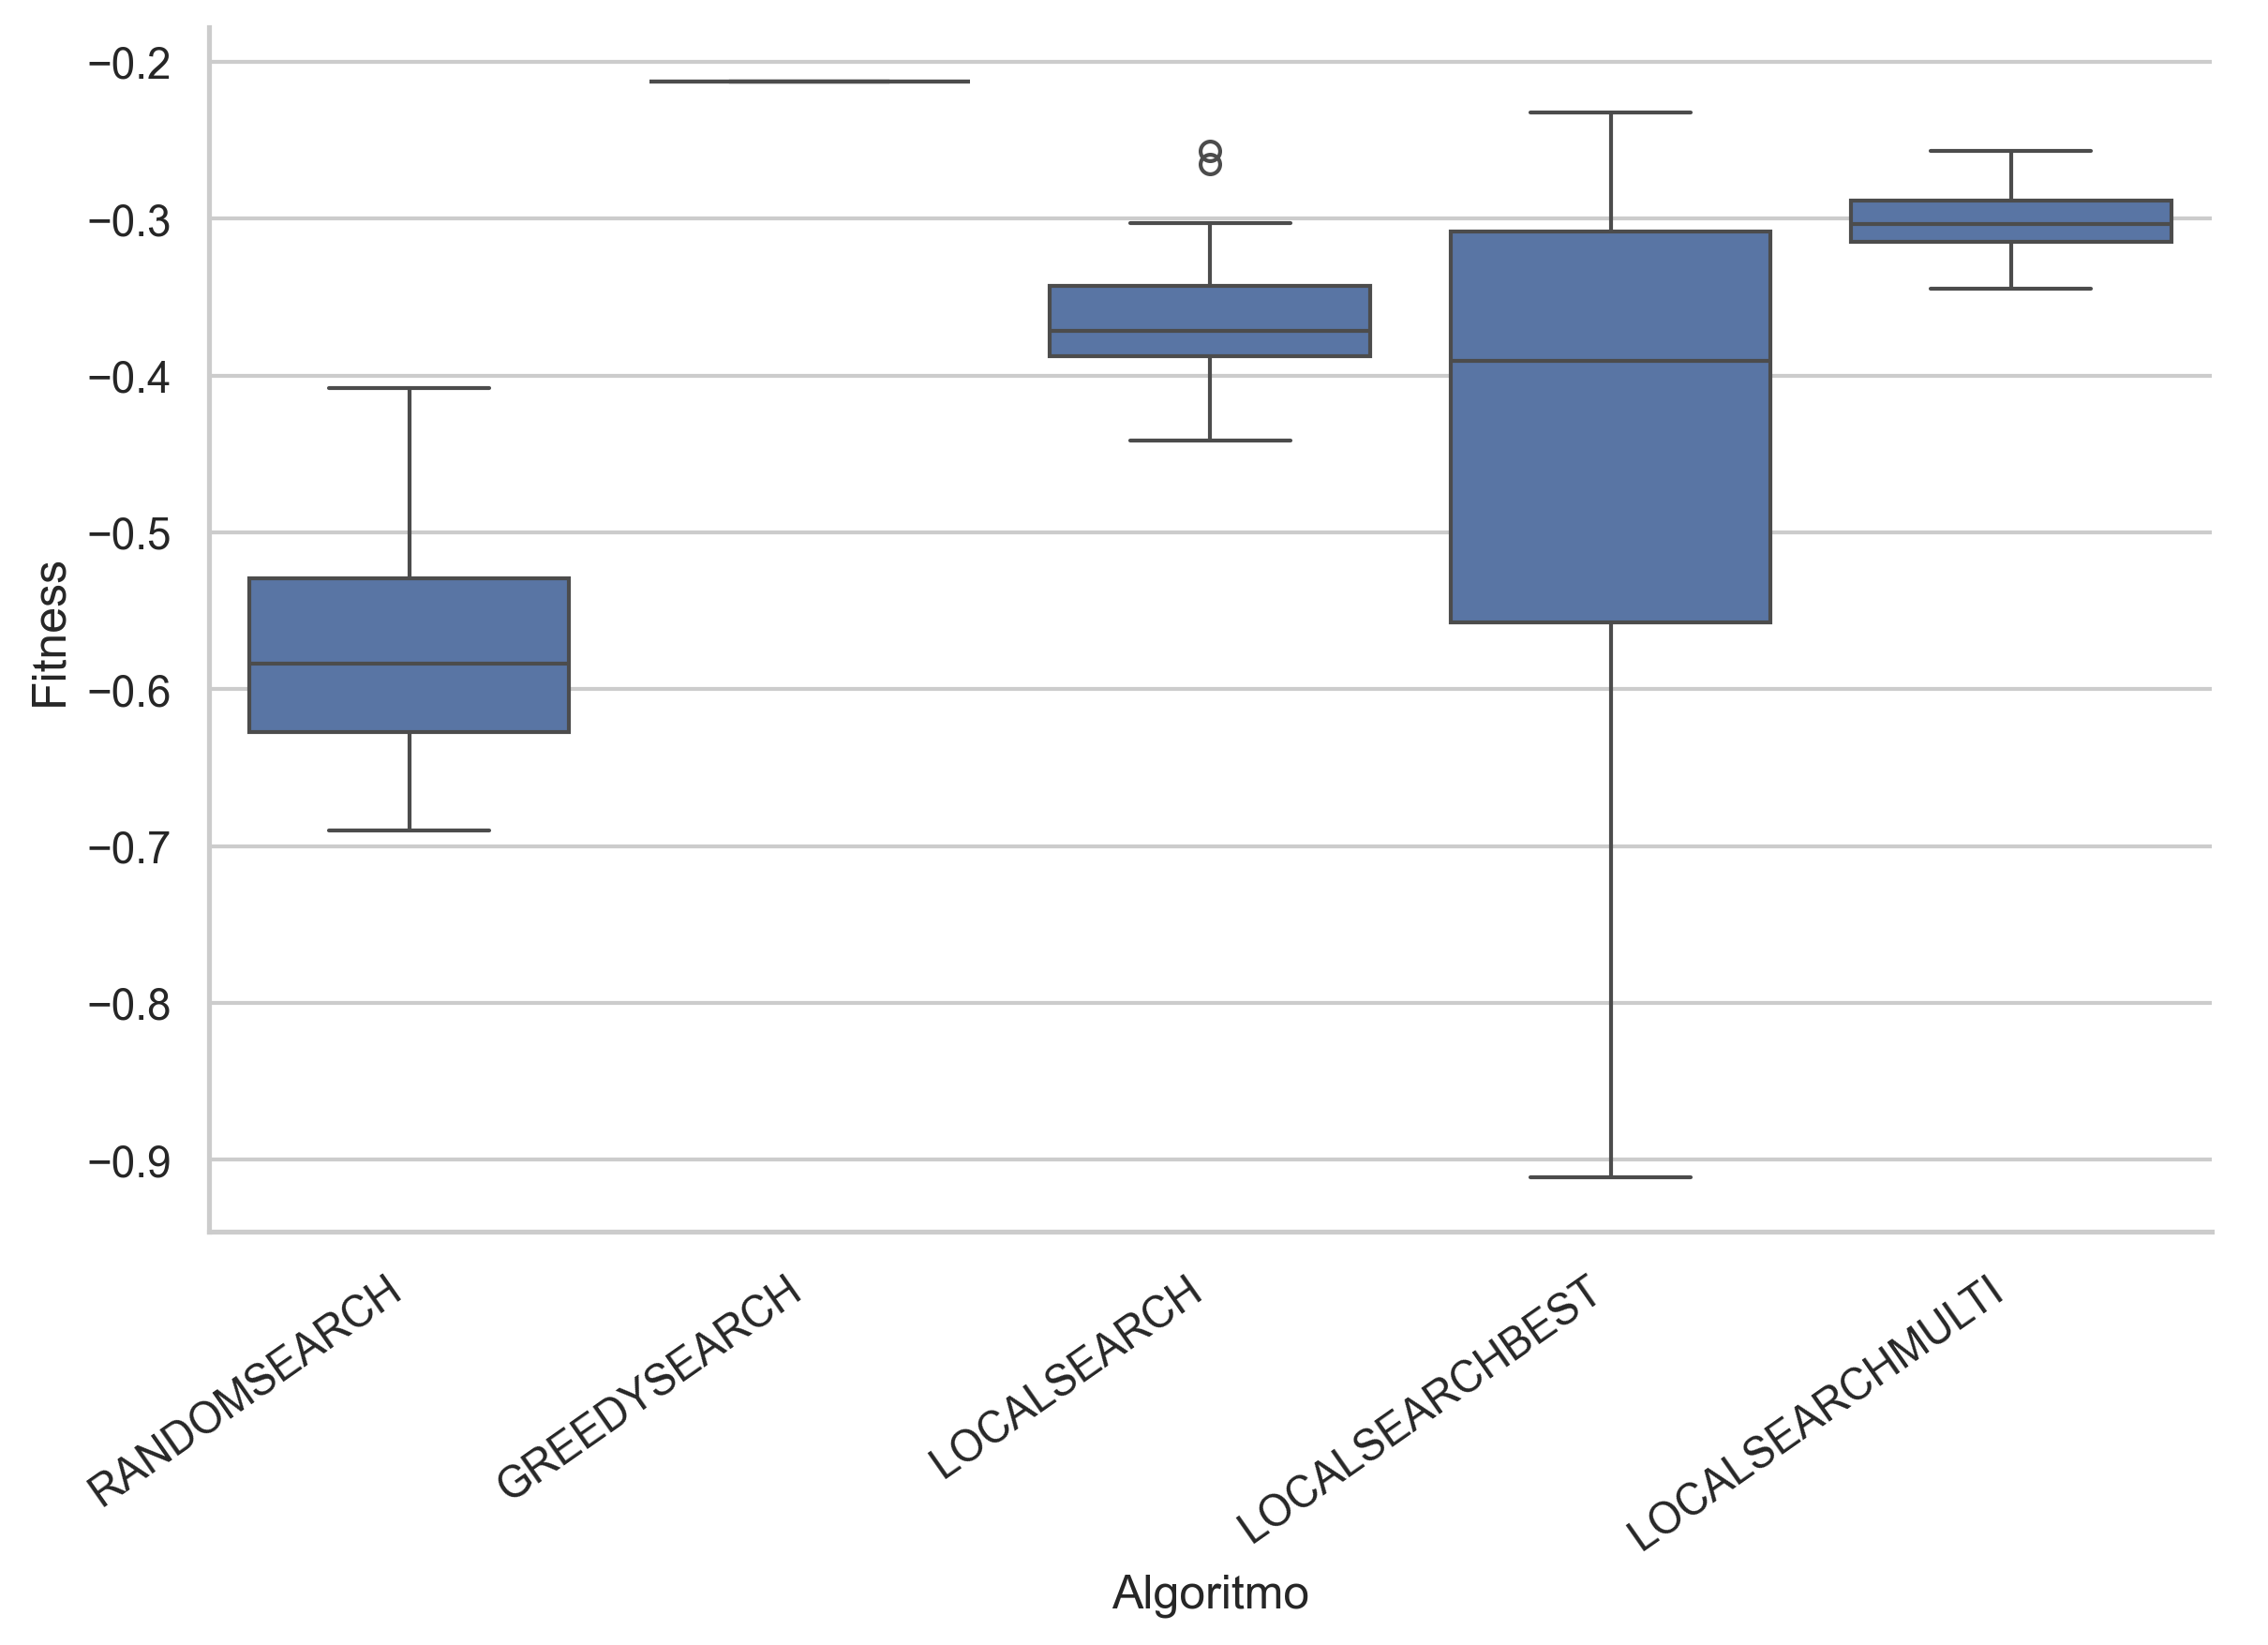
\includegraphics[width=0.7\textwidth]{figuras/IBEX_35_resultados.png}
    \caption{Distribución de Fitness en Train (50 ejecuciones) para el IBEX 35 ($N=30$).}
    \label{fig:boxplot_ibex}
\end{figure}

El boxplot del IBEX 35 (Figura \ref{fig:boxplot_ibex}) ilustra perfectamente la jerarquía de los algoritmos. El \textbf{Greedy Search} se visualiza como una línea plana en la cota superior, marcando el techo de rendimiento histórico (dado su carácter determinista, carece de varianza). Sin embargo, dentro de los métodos estocásticos (aquellos que generalizan mejor a futuro), la \textbf{BL Multiarranque} demuestra una clara superioridad estadística. Su caja se sitúa de forma consistente por encima de la BL estándar y de la Búsqueda Aleatoria. Por el contrario, la \textbf{BL del Mejor} queda relegada a la zona inferior, reflejando su incapacidad para avanzar en el espacio de búsqueda debido al coste excesivo de evaluar el vecindario completo en cada iteración.

\begin{figure}[H]
    \centering
    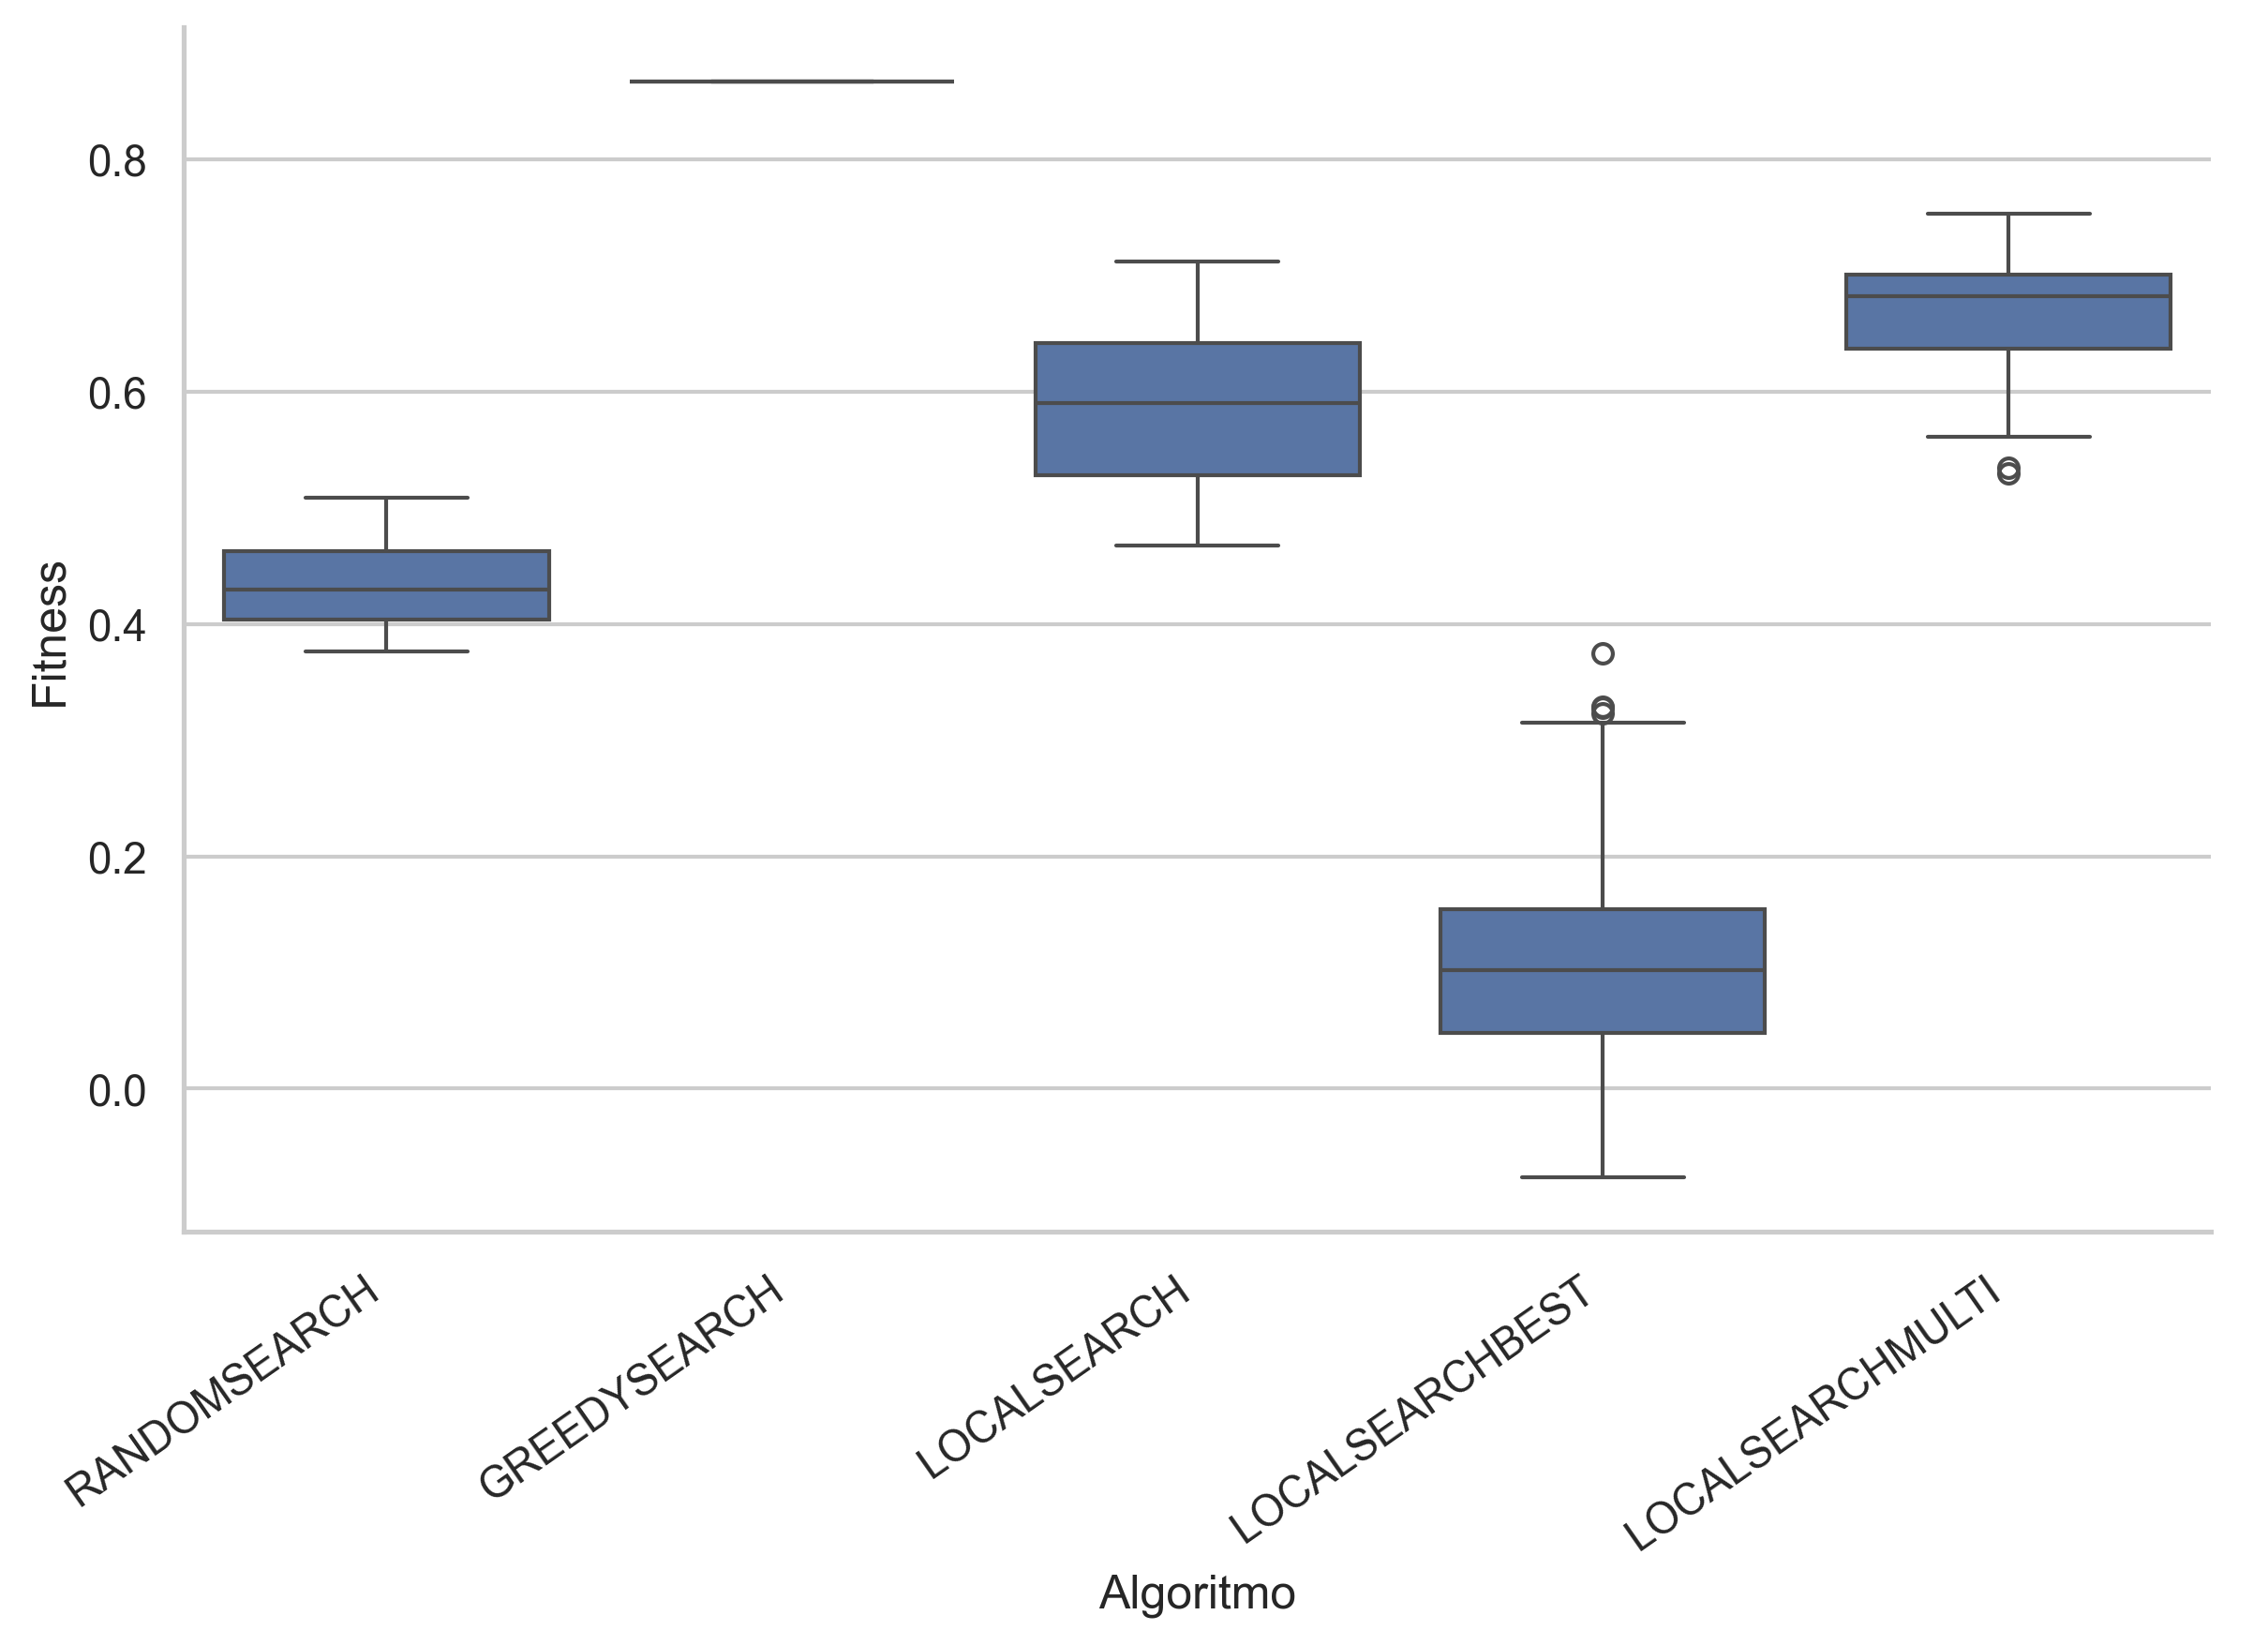
\includegraphics[width=0.7\textwidth]{figuras/S_P_100_resultados.png}
    \caption{Distribución de Fitness en Train (50 ejecuciones) para el S\&P 100 ($N=97$).}
    \label{fig:boxplot_sp100}
\end{figure}

En el S\&P 100 (Figura \ref{fig:boxplot_sp100}), la tendencia se agudiza. Mientras el algoritmo Greedy sigue coronando la gráfica con el máximo ajuste a los datos históricos, la \textbf{BL Multiarranque} se consolida como la trayectoria exploratoria más eficiente, separándose notablemente de la BL del Primer Mejor. Es especialmente revelador el hundimiento de la \textbf{BL del Mejor}, cuya caja desciende hasta solaparse con la \textbf{Búsqueda Aleatoria}. Esto confirma visualmente el diagnóstico matemático: el algoritmo agota su presupuesto evaluando el vecindario inicial, sin lograr dar pasos reales de mejora.

\begin{figure}[H]
    \centering
    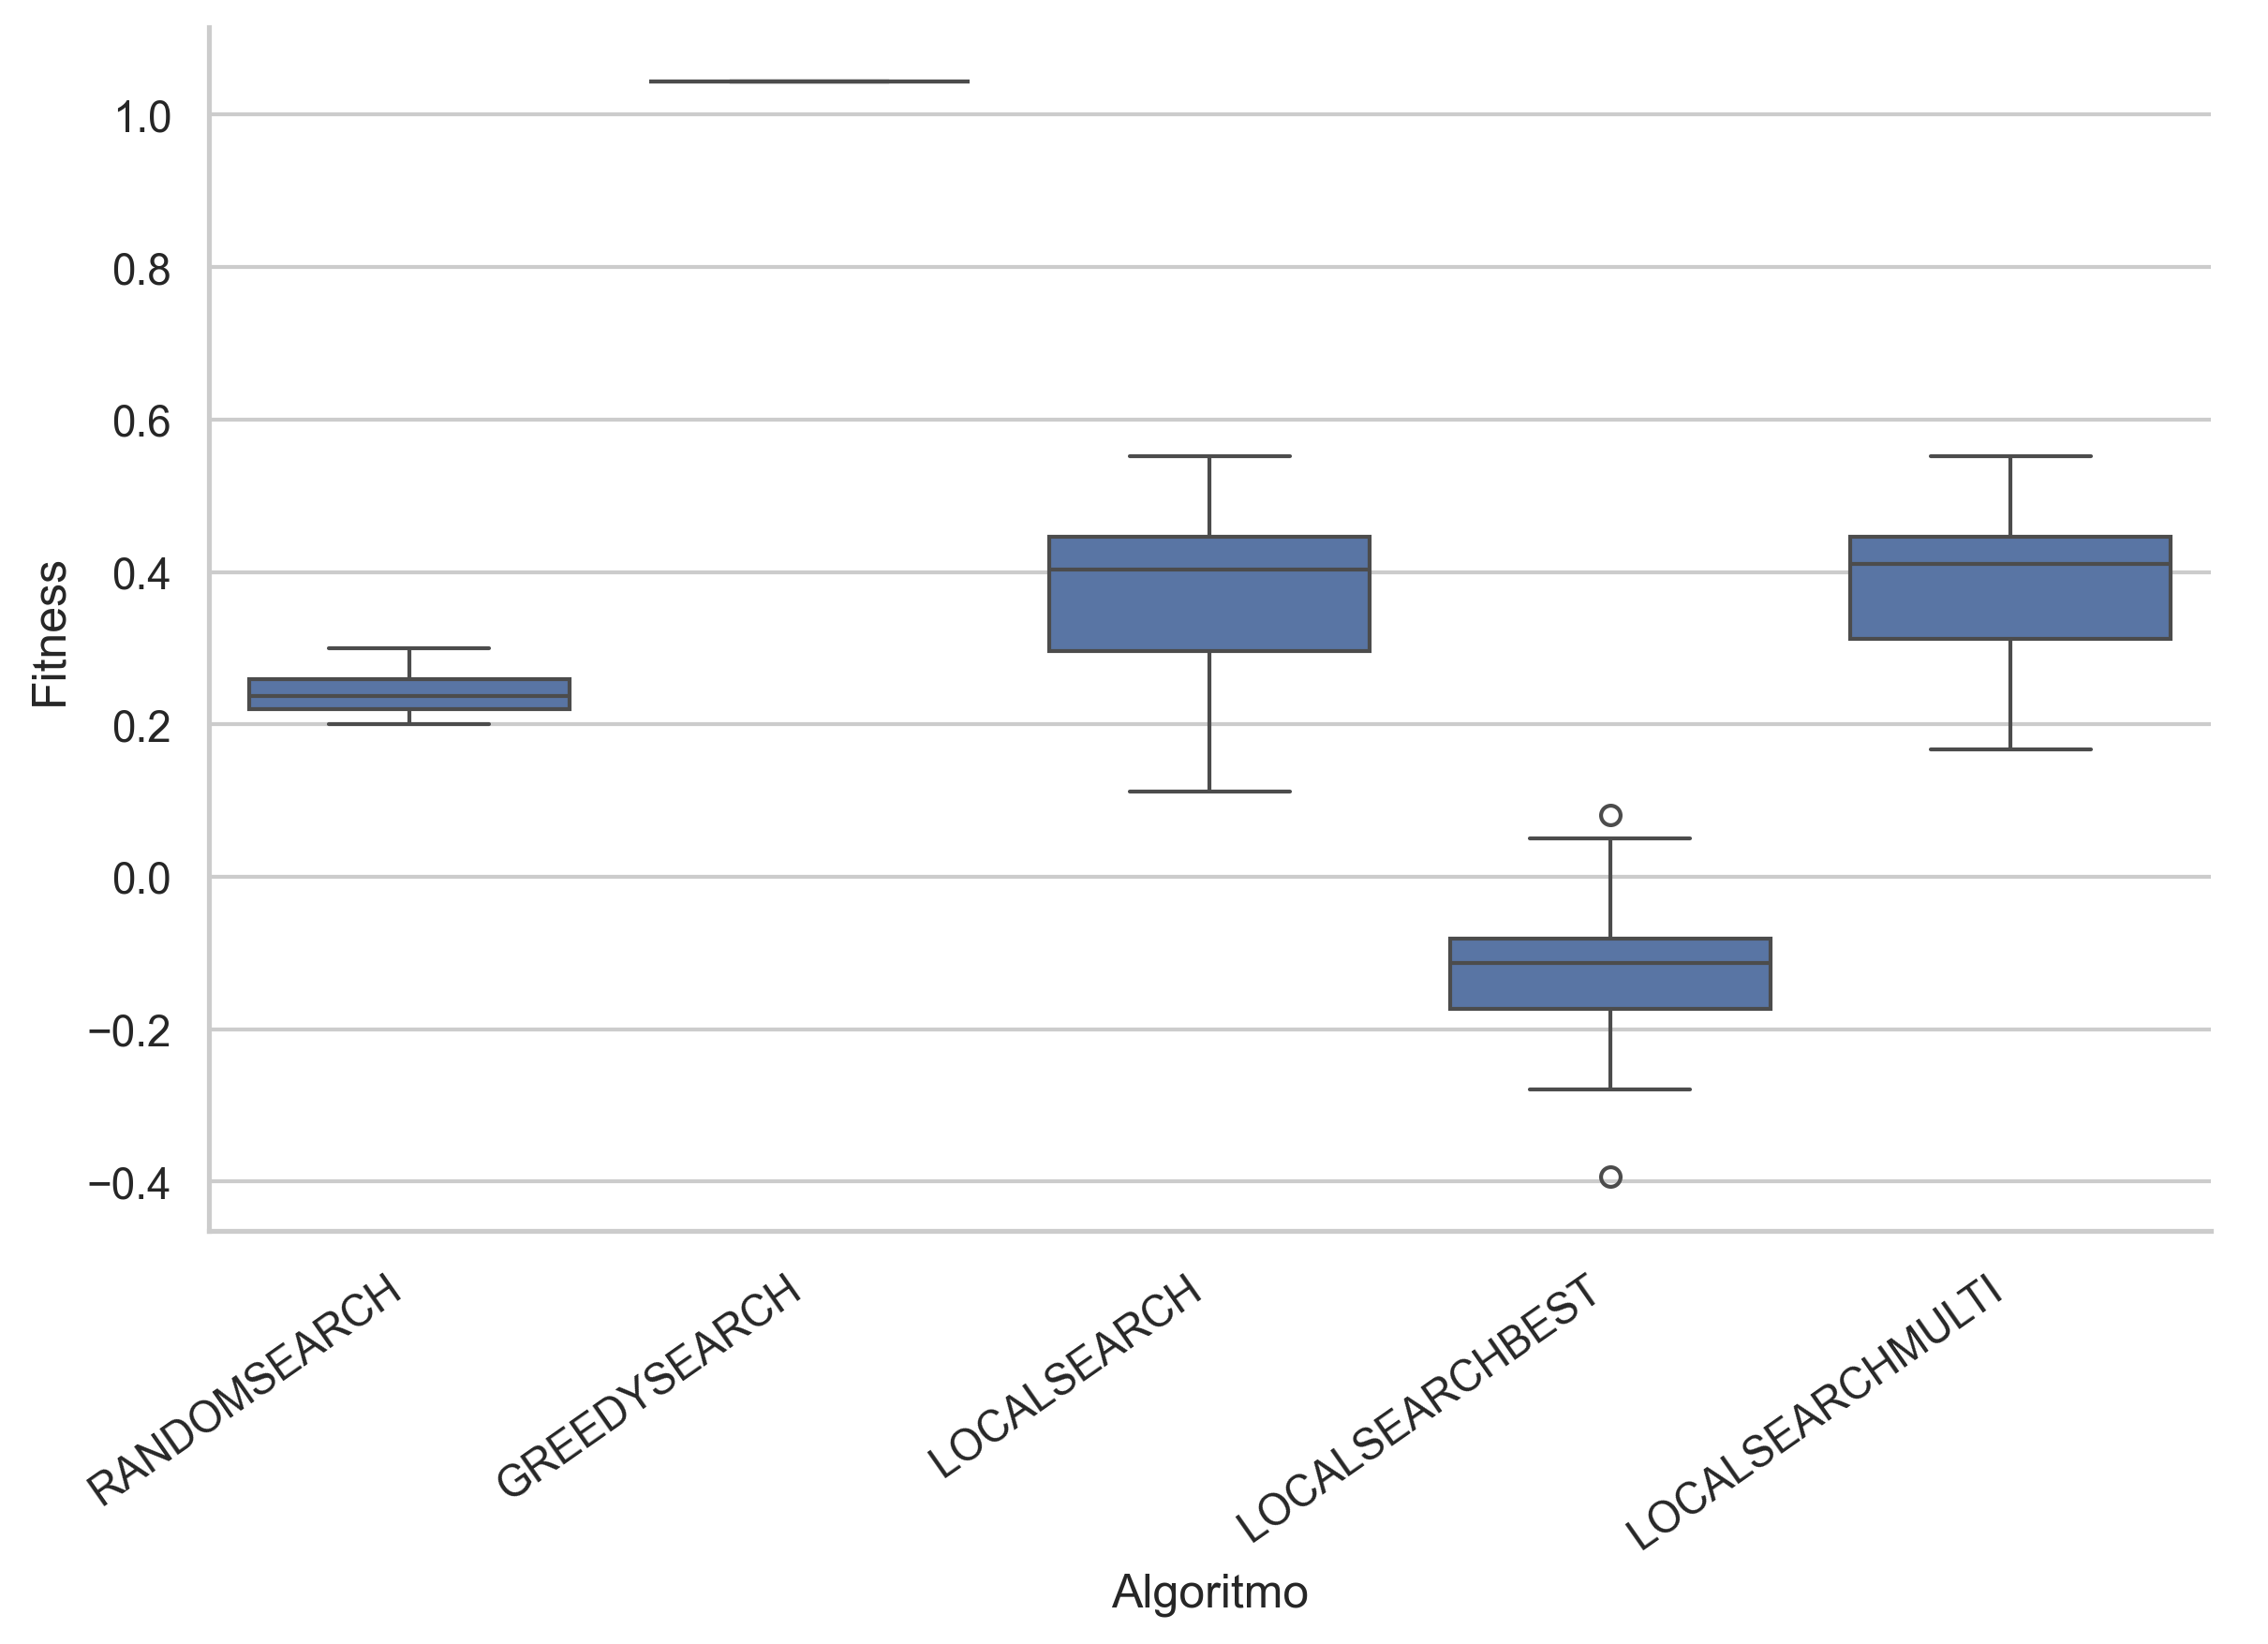
\includegraphics[width=0.7\textwidth]{figuras/S_P_500_resultados.png}
    \caption{Distribución de Fitness en Train (50 ejecuciones) para el S\&P 500 ($N=457$).}
    \label{fig:boxplot_sp500}
\end{figure}

Finalmente, el gráfico del S\&P 500 (Figura \ref{fig:boxplot_sp500}) ofrece la visualización más clara sobre los límites de escalabilidad. Obviando el pico determinista del Greedy, las cajas de la \textbf{BL Multiarranque} y la \textbf{Búsqueda Local estándar} (Primer Mejor) son prácticamente idénticas. Esto ilustra el fenómeno de la inanición por evaluaciones: una sola ejecución de la BL ya consume casi la totalidad de las 10.000 evaluaciones permitidas, dejando al Multiarranque sin margen para reiniciar el proceso. La \textbf{BL del Mejor} desaparece por completo de la zona competitiva, hundida en valores negativos por su inmovilismo.

\textbf{Conclusión:} La comparativa visual confirma que, descartando el sobreajuste masivo del enfoque Greedy, la Búsqueda Local Multiarranque es la estrategia estocástica dominante. Su eficacia depende directamente de que el ratio entre el presupuesto de evaluaciones y la dimensión del problema permita múltiples reinicios efectivos.

\subsection{Arquitectura de Configuración Dinámica}

Como aportación voluntaria de ingeniería de software, se ha diseñado e integrado un módulo \texttt{ConfigReader} que desacopla completamente la parametrización experimental del código fuente C++. Este componente permite cargar en tiempo de ejecución, desde el fichero \texttt{config.cfg}, tanto los hiperparámetros del experimento como las decisiones de selección de datos.

En particular, la arquitectura implementada permite modificar sin recompilar:
\begin{itemize}
    \item el tamaño del salto de la Búsqueda Local mediante \texttt{LS\_RATIO},
    \item la penalización del riesgo del modelo de Markowitz mediante el parámetro $\lambda$,
    \item y los datasets a evaluar, pudiendo alternar entre los tres mercados por defecto o activar un mercado personalizado (\textit{Custom Market}).
\end{itemize}

Este diseño aporta flexibilidad, escalabilidad y trazabilidad experimental: los cambios de escenario se realizan editando únicamente el archivo de configuración, evitando introducir ``números mágicos'' en el código y reduciendo el coste de mantenimiento para nuevas campañas de experimentación.
